\documentclass{article}
\usepackage{graphicx}
\usepackage{amsmath, amssymb, float}
\usepackage{tikz}
\usetikzlibrary{angles,quotes}

\DeclareMathOperator{\EX}{\mathbb{E}}% expected value
\DeclareMathOperator{\Var}{\operatorname{Var}}% variance
\DeclareMathOperator{\Span}{\operatorname{span}}% span

\title{Tech Talk Notes}
\author{rlybrdgs }

\begin{document}

\maketitle
\begin{enumerate}
    \item Common Pose Operations:
    \begin{align*}
        P^A_B \cdot P^B_C &= P^A_C \\
        \left(P^A_B\right)^{-1} &= P^B_A \\
        T^A_B \cdot v_A &= v_B \\
    \end{align*}

    \item Position Operations:
    \begin{align*}
        \begin{bmatrix}
            x \\ y \\ z
        \end{bmatrix} \quad \begin{bmatrix}
            x \\ y
        \end{bmatrix} \\
        p^A_B + p^B_C &= p^A_C \\
        -p^A_B &= p^B_A \\
        p^A_B + p_A &= p_B \\
    \end{align*}

    \item commutative:
    \begin{align*}
        R_1 \cdot R_2 &= R_2 \cdot R_1 \\
        R_1 \cdot R_2 &\neq R_2 \cdot R_1 \\
    \end{align*}

    \item Rotation Matrix:
    \begin{align*}
        R &= \begin{bmatrix}
            r_{11} & r_{12} \\ r_{21} & r_{22}
        \end{bmatrix} \\
        z = a + bi, \quad \sqrt{a^2 + b^2} &= 1 \\
        R &= \begin{bmatrix}
            r_{11} & r_{12} & r_{13} \\ r_{21} & r_{22} & r_{23} \\ r_{31} & r_{32} & r_{33} 
        \end{bmatrix} \\
        R &= \begin{bmatrix}
            \begin{bmatrix}
                r_{11} \\ r_{21} \\ r_{31}
            \end{bmatrix} & \begin{bmatrix}
                r_{12} \\ r_{22} \\ r_{32}
            \end{bmatrix} & \begin{bmatrix}
                r_{13} \\ r_{23} \\ r_{33}
            \end{bmatrix}
        \end{bmatrix} \\
        \begin{bmatrix}
            v_1 & v_2 & v_3
        \end{bmatrix}^\top \cdot \theta \\
        v \quad p \quad p_{\text{rot}} \\
        \mathbf{q} &= \begin{bmatrix}
            x & y & z & w
        \end{bmatrix}^\top = w + x\mathbf{i} + y\mathbf{j} + z\mathbf{k} \\
        \mathbb{S}^3
    \end{align*}

    \item Pose Operations:
    \begin{align*}
        M &= \begin{bmatrix}
            R & t \\ 0 & 1
        \end{bmatrix} = \begin{bmatrix}
            r_{11} & r_{12} & r_{13} & t_x \\ r_{21} & r_{22} & r_{23} & t_y \\ r_{31} & r_{32} & r_{33} & t_z \\ 0 & 0 & 0 & 1
        \end{bmatrix} \\
        M_1 M_2 &= \begin{bmatrix}
            R_1 & t_1 \\ 0 & 1
        \end{bmatrix} \begin{bmatrix}
            R_2 & t_2 \\ 0 & 1
        \end{bmatrix} \\
        &= \begin{bmatrix}
            R_1 R_2 & R_1 t_2 + t_1 \\ 0 & 1
        \end{bmatrix}
    \end{align*}

    \item 2D diagrams:
    \begin{tikzpicture}
        \def\r{1.5}
        \def\mtheta{30}
        \coordinate (o) at (0,0);
        \coordinate (r) at ({\r*cos(\mtheta)}, {\r*sin(\mtheta)});
        \coordinate (x) at (1,0);
        \draw[thick, <->] (-2,0) -- (2,0) node[right] {$x$}; 
        \draw[thick, <->] (0,-2) -- (0,2) node[above] {$y$};
        \draw[very thick, red, ->] (o) -- (r) node[right] {object}; 
        \pic[draw, thick, ->, "$\theta$", angle eccentricity=1.5] {angle = x--o--r};
    \end{tikzpicture}

    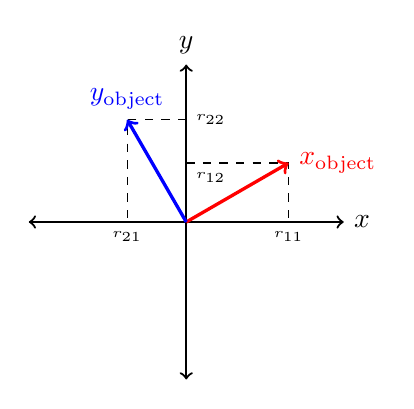
\begin{tikzpicture}
        % \draw[very thin,color=gray] (-3,-3) grid (3,3);
        \def\r{1.5}
        \def\range{2}
        \def\mtheta{30}
        \coordinate (o) at (0,0);
        \coordinate (r) at ({\r*cos(\mtheta)}, {\r*sin(\mtheta)});
        \coordinate (v) at ({-\r*sin(\mtheta)}, {\r*cos(\mtheta)});
        \coordinate (x) at (1,0);
        \draw[thick, <->] (-\range,0) -- (\range,0) node[right] {$x$}; 
        \draw[thick, <->] (0,-\range) -- (0,\range) node[above] {$y$};
        \draw[dashed] (o|-r) node[anchor=north west]{\tiny $r_{12}$} -- (r) -- (r|-o) node[below]{\tiny $r_{11}$};
        \draw[dashed] (o|-v) node[right]{\tiny $r_{22}$} -- (v) -- (v|-o) node[below]{\tiny $r_{21}$};
        \draw[very thick, red, ->] (o) -- (r) node[right] {$x_{\text{object}}$}; 
        \draw[very thick, blue, ->] (o) -- (v) node[above] {$y_{\text{object}}$};
        % \pic[draw, thick, ->, "$\theta$", angle eccentricity=1.5] {angle = x--o--r};
    \end{tikzpicture}

    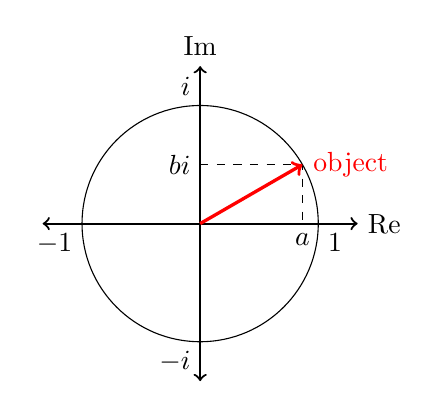
\begin{tikzpicture}
        \def\r{1.5}
        \def\mtheta{30}
        \coordinate (o) at (0,0);
        \coordinate (r) at ({\r*cos(\mtheta)}, {\r*sin(\mtheta)});
        \coordinate (x) at (\r,0);
        \coordinate (y) at (0,\r);
        \draw[] (o) circle (\r);
        \draw[thick,<->] (-2,0) -- (2,0) node[right] {Re}; 
        \draw[thick, <->] (0,-2) -- (0,2) node[above] {Im};
        \draw[dashed] (o|-r) node[left]{$bi$} -- (r) -- (r|-o) node[below]{$a$};
        \draw[very thick, red, ->] (o) -- (r) node[right] {object};
        \draw (\r,0) node[anchor=north west] {$1$};
        \draw (-\r,0) node[anchor=north east] {$-1$};
        \draw (0,\r) node[anchor=south east] {$i$};
        \draw (0,-\r) node[anchor=north east] {$-i$};
    \end{tikzpicture}
\end{enumerate}

\end{document}